%%---------------------------------------------------------------------------%%
\section{Description of the numerical models}
\label{sec:model}

In this section we discuss the numerical setup related to the full core simulations performed.
The full core configuration used is the one provided in a previous publication. A schematic of the core is provided in Figure~\ref{fig:core} featuring 37 identical assemblies. The assembly design is identical to what discussed in previous publications with a 17x17 configuration \cite{merzari2020wall}.

\begin{figure}[!ht]
\centering
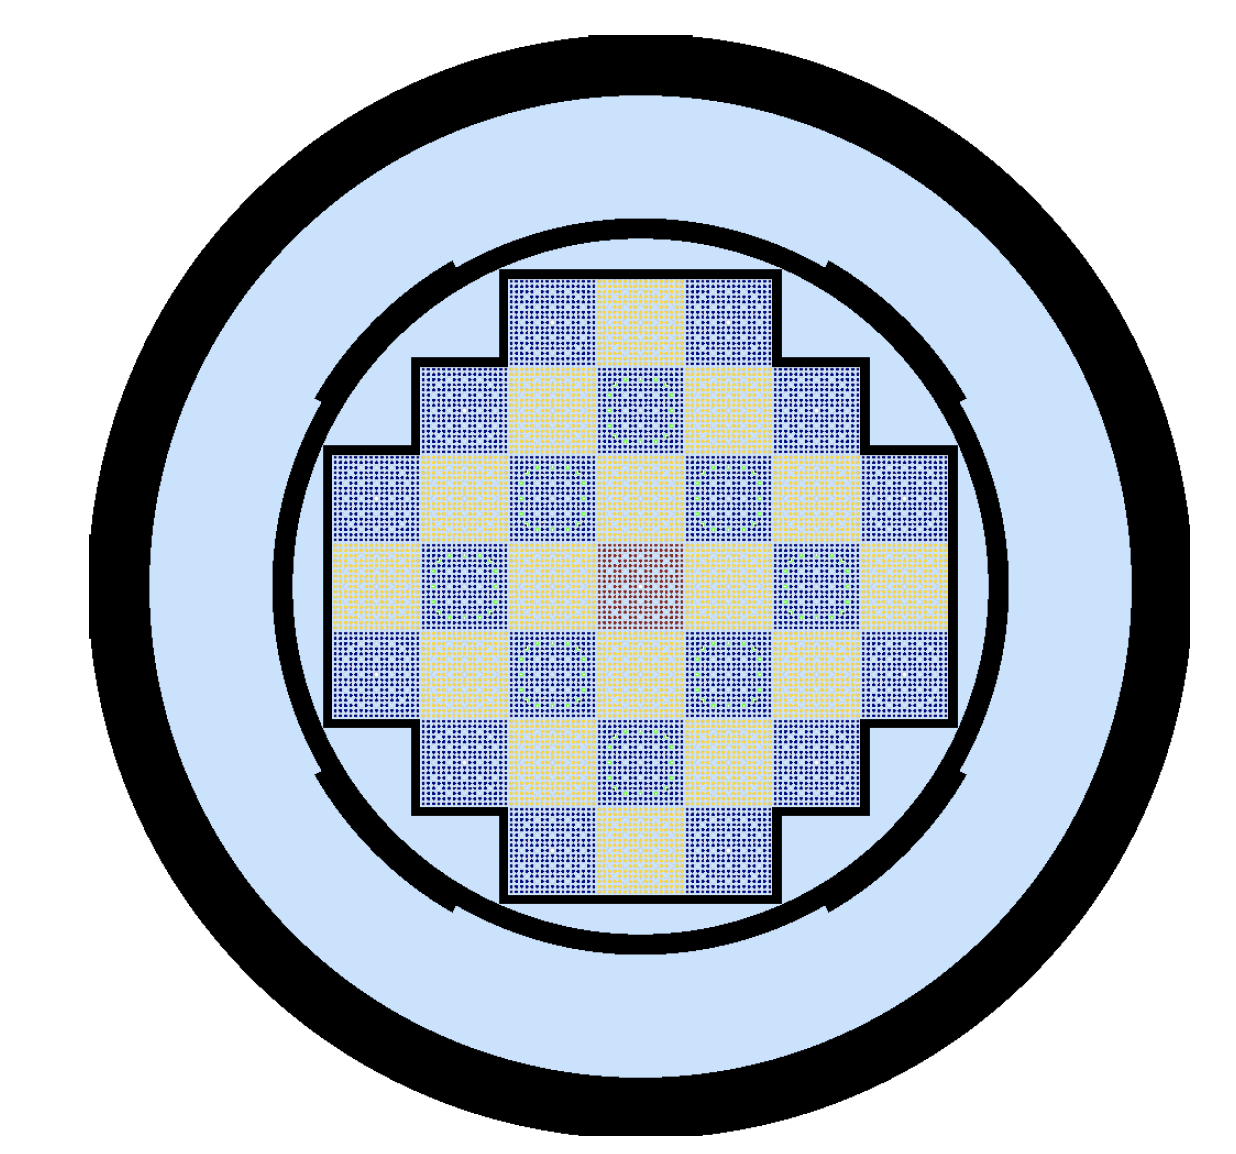
\includegraphics[width=0.5\textwidth]{./figures/core_slice.png}
\caption{Core slice showing the geometry.}
\label{fig:core}
\end{figure}

All calculations performed as part of the full core simulation campaign use the same base 2D fluid mesh, which is then extruded in the axial direction. Each fluid layer contains over a million elements. The conjugate heat transfer case examined has also mesh for the cladding, the gap and the rods, and each CHT layer contains over 2 million elements. The GLL points at polynomial order $N=2$ obtained from the mesh devised for the fluid portion of the domain is shown in Figure~\ref{fig:mesh1}.

\begin{figure}[!ht]
\centering
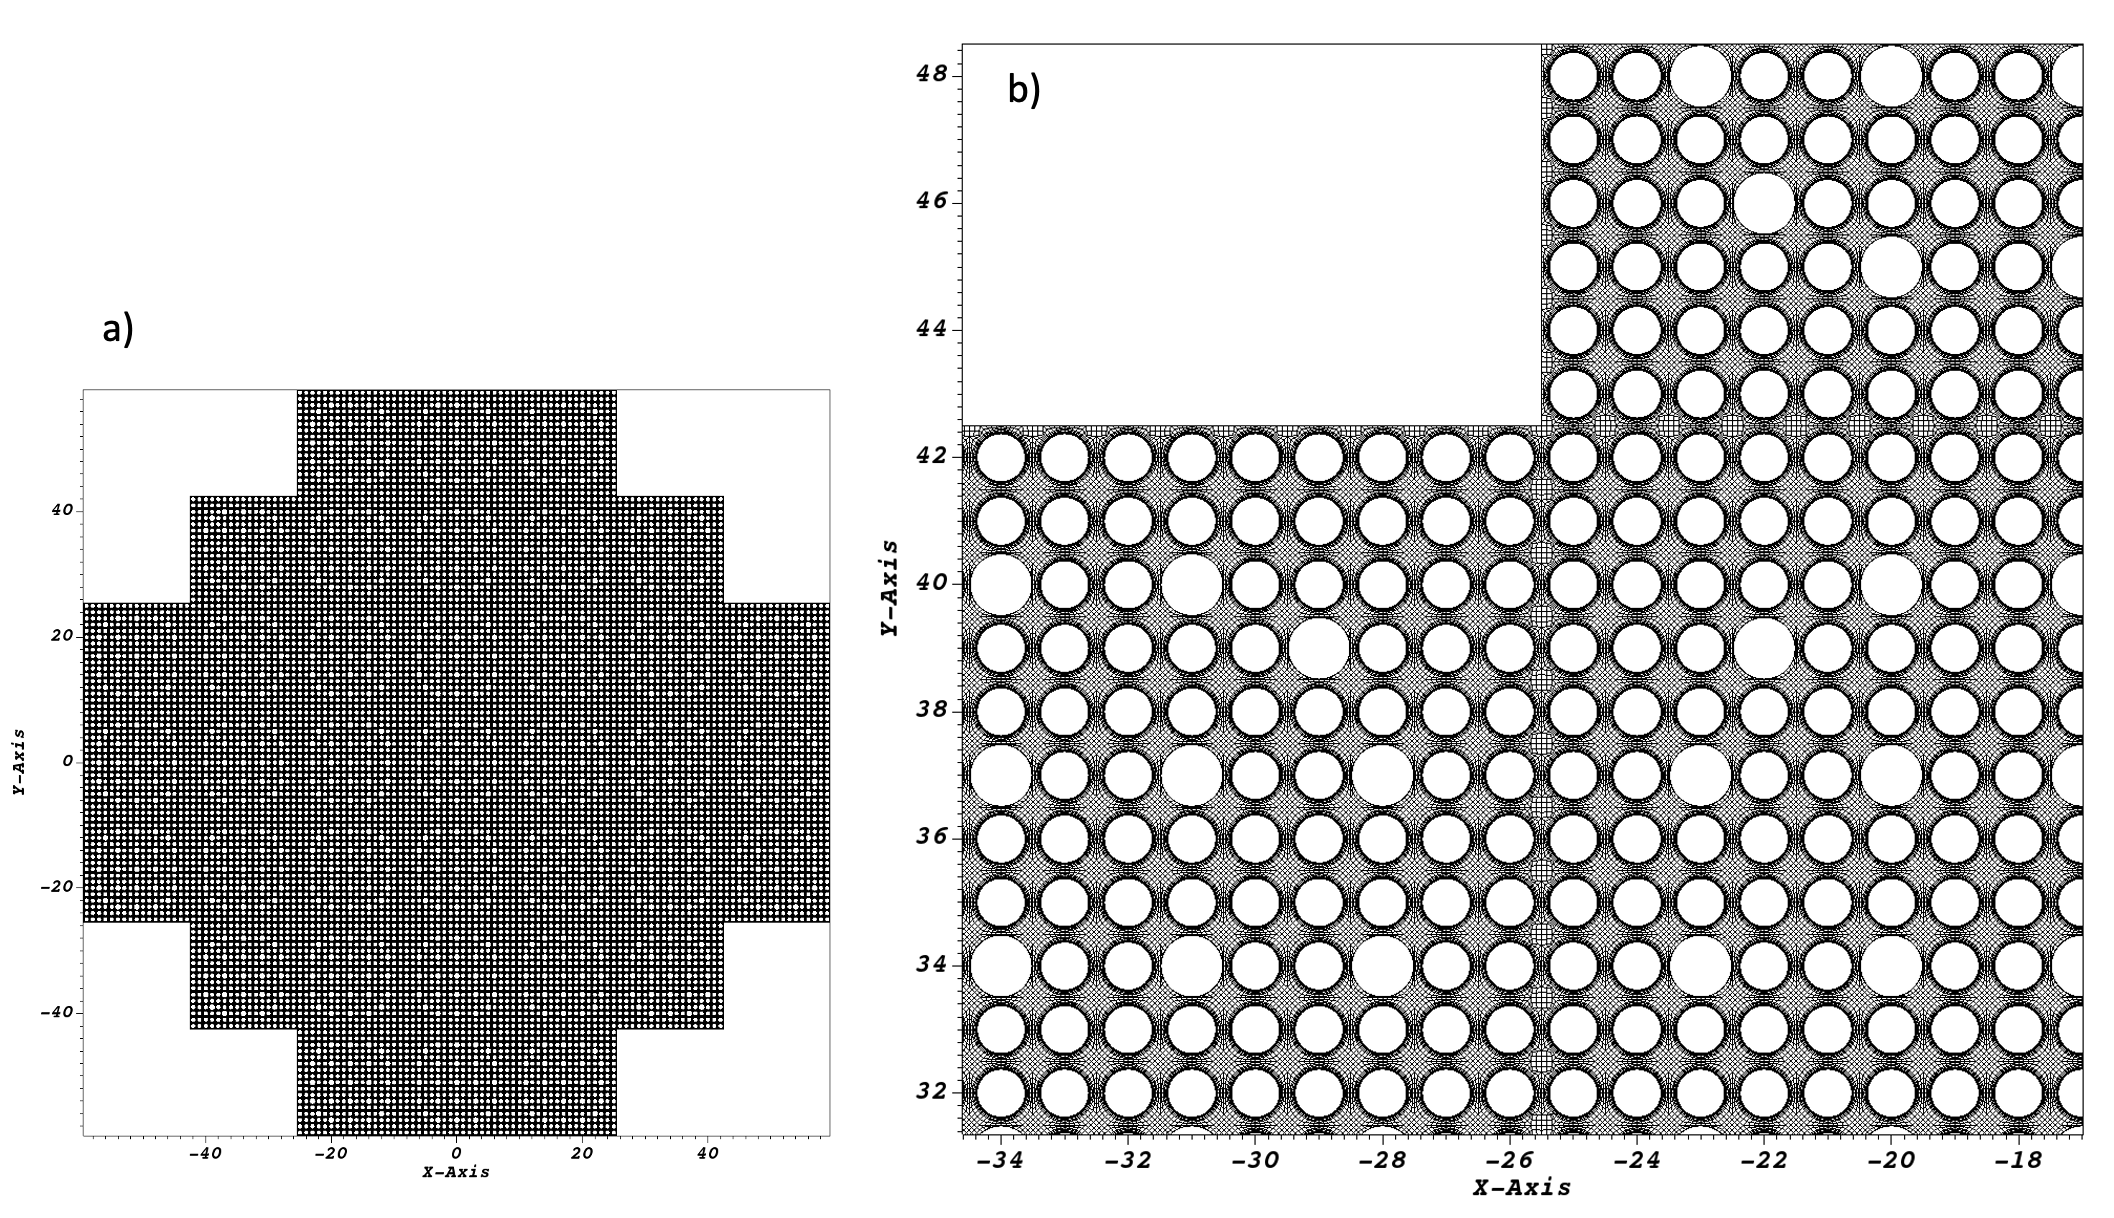
\includegraphics[width=0.99\textwidth]{./figures/full_core_mesh.png}
\caption{Mesh for the full core simulations. 2D section at low polynomial order. a) full core, b) detail.}
\label{fig:mesh1}
\end{figure}

Table~\ref{tab:full core} includes data for six representative cases, as part of this simulation campaign. Cases III and V represent full height core simulations with and without momentum sources performed with RANS. Case VI represent an initial simulation performed with Conjugate heat transfer. Most cases involve inlet/outlet boundary conditions. Case I is the case used the updated FOM calculation for ExaSMR.

\begin{table} \centering \small
% \resizebox{0.48\textwidth}{!}{
 \begin{tabular}{ccccc} \hline \hline
  Case & Boundary conditions & Model & Number of Layers $n$ & Grid points \\ \hline
   I & inlet/outlet & Large Eddy Simulation & 174 & $59.8 \cdot 10^{9}$ \\
   II & periodic slice & RANS & 3 & $1.1 \cdot 10^{9}$ \\
   III & inlet/outlet & RANS & 100 & $35.8 \cdot 10^{9}$ \\
   IV & inlet/outlet & Momentum sources, RANS & 15 & $5.2 \cdot 10^{9}$ \\
   V & inlet/outlet & Momentum sources, RANS & 100 & $35.8 \cdot 10^{9}$ \\
   VI & inlet/outlet & Conjugate Heat Transfer & 50 & $38.8 \cdot 10^{9}$ \\
   \hline \hline
\end{tabular}
 \caption{Full core cases performed: description of setup}
 \label{tab:full core}
\end{table}
